\documentclass{beamer}

\usepackage{fontspec}
\usepackage{xeCJK}
\setCJKmainfont[BoldFont=Noto Serif CJK TC Bold]{Noto Serif CJK TC}
\XeTeXlinebreaklocale "zh"
\XeTeXlinebreakskip = 0pt plus 1pt
\linespread{1.3}
\allowdisplaybreaks

\usepackage{color}
\usepackage{booktabs}
\usepackage{tabularx}
\usepackage{caption}
\usepackage{tikz}
\usepackage{verbatim}
\usepackage{pgfplotstable}
\pgfplotsset{width=12cm}
\pgfplotsset{height=7cm}
\pgfplotsset{compat=1.13}

\usetheme{EastLansing}
\usetikzlibrary{positioning}
\useinnertheme{rectangles}
\usefonttheme{professionalfonts}

\newcommand{\lw}{0.8mm}
\setbeamercovered{transparent}


%\AtBeginSection[]
%{
  %\begin{frame}<beamer>
	%\frametitle{報告大綱}
	%%\frametitle{RoadMap}
    %\tableofcontents[currentsection]
  %\end{frame}
%}

\title{Paper Report}
\subtitle{\textcolor[rgb]{0.00,0.50,1.00}{{Speech Processing \& Machine Learning Laboratory}}}
\author{徐瑞陽}
\date{2020/04/08}
\begin{document}

\begin{frame}
\maketitle
\end{frame}




%\begin{frame}[t]{Domain Generalization in Meta Learning}
%\end{frame}

\begin{frame}
  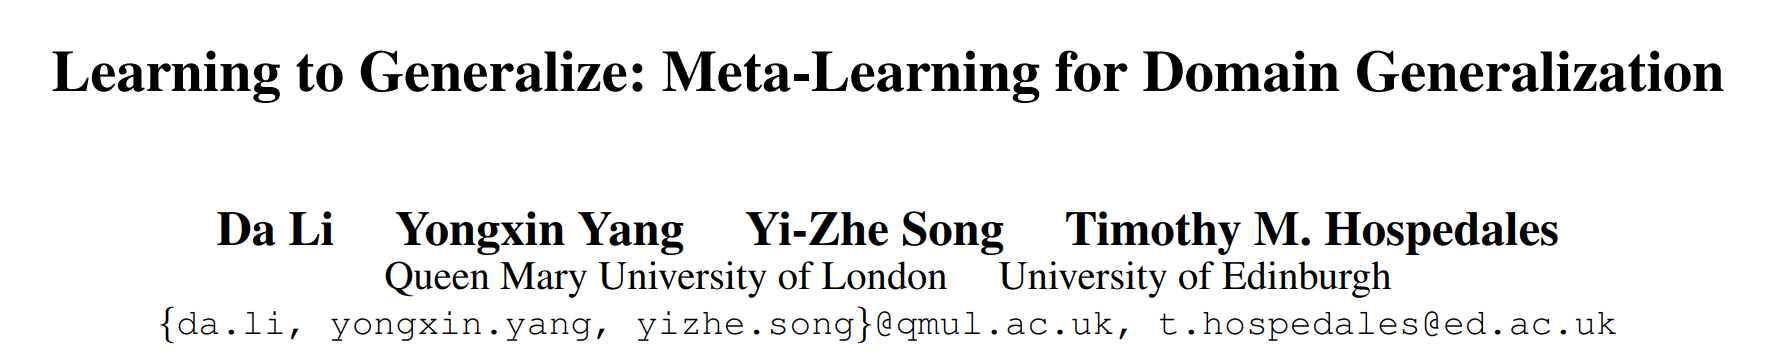
\includegraphics[width=\textwidth]{fig/MLDG-title.png}
  \center AAAI 2018
\end{frame}

\begin{frame}
  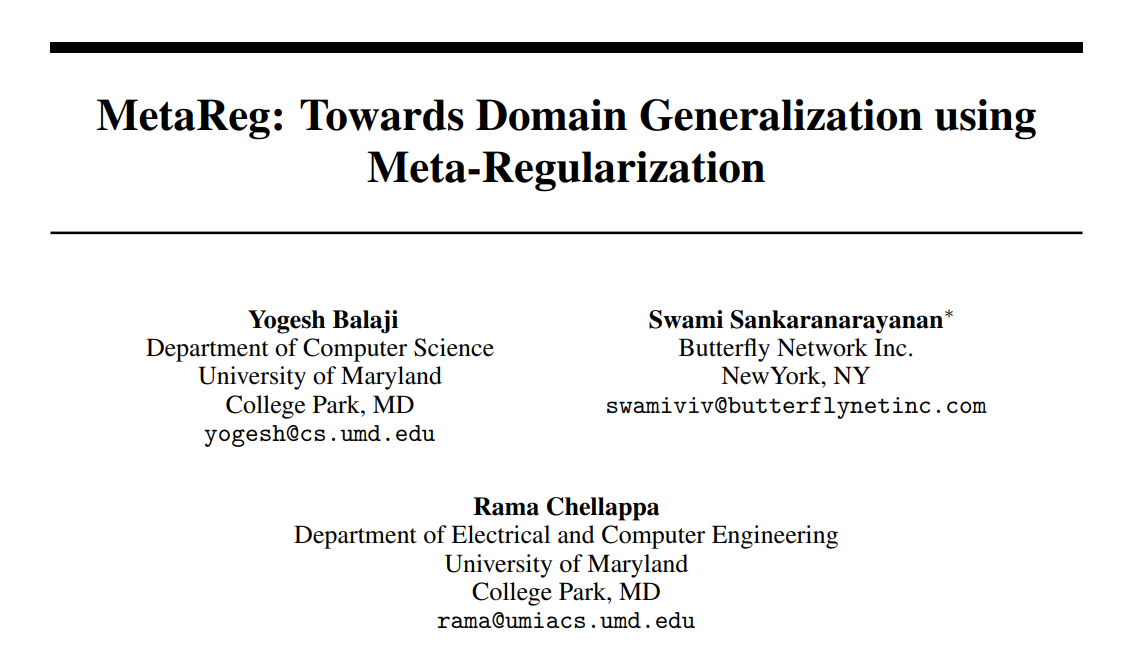
\includegraphics[width=\textwidth]{fig/MetaReg.png}
  \center NeurIPS 2018
\end{frame}

\begin{frame}
  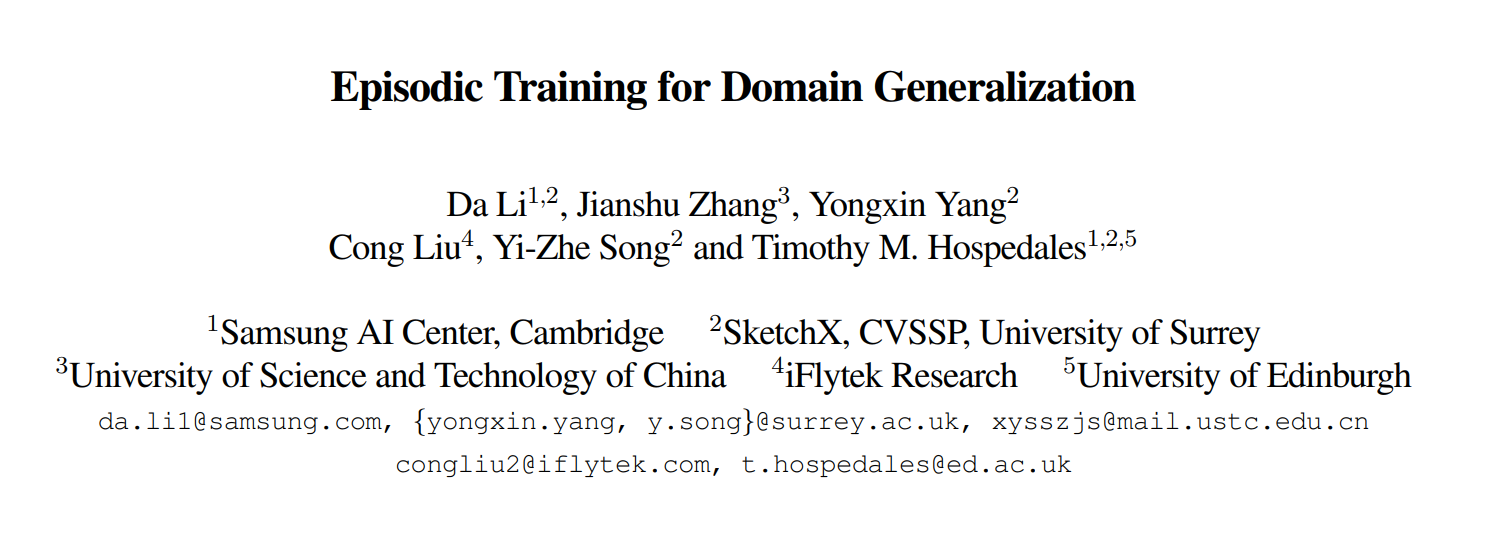
\includegraphics[width=\textwidth]{fig/EpiFCR-title.png}
  \center ICCV 2019
\end{frame}

\begin{frame}
\frametitle{Outline}
\tableofcontents
\end{frame}

\section{Quick Recap of Meta Learning}
\begin{frame}{Objective}
      \begin{equation*}
        \theta^{\star} = \arg \max_\theta \mathbb{E}_{\mathcal{D} \sim p(\mathcal{D}) }[\mathcal{A}_{f_\theta(\mathcal{D^{\text{tr}}})}(\mathcal{D^{\text{test}}})]
      \end{equation*}

      \begin{itemize}
        \item $f_\theta: \mathcal{D} \rightarrow M$, meta model
        \item $\mathcal{A}_M(\mathcal{D}): $ goodness function of model $M$ on $\mathcal{D}$
      \end{itemize}
\end{frame}

\begin{frame}[t]{Different implementations of $f_\theta$}
  \begin{itemize}
    \item Metric-based: e.g. ProtoNet
    \item Model-based (Blackbox Adaptation): e.g. SNAIL
    \item \textbf{Gradient-based}: e.g. MAML, Reptile
  \end{itemize}
\end{frame}

\begin{frame}[t]{Properties meta-model $f_\theta$ should have}
      \begin{equation*}
        \theta^{\star} = \arg \max_\theta \mathbb{E}_{\mathcal{D} \sim p(\mathcal{D}) }[\mathcal{A}_{f_\theta(\mathcal{D^{\text{tr}}})}(\mathcal{D^{\text{test}}})]
      \end{equation*}

      \begin{itemize}
        \item $f_\theta$ can utilize task information MORE $\rightarrow$ my report in 2019/09
          \begin{itemize}
            \item \textbf{Task Conditioning}: utilize prior information about tasks to adjust shared parameter
            \item \textbf{Parameter Space Warping}: meta learn which part of model should share
          \end{itemize}

        \item $f_\theta$ can also do well in $\mathcal{D}$ which is out-of-domain (OOD)
          \begin{itemize}
            \item Domain Adaptation
            \item \textbf{Domain Generalization}
          \end{itemize}
      \end{itemize}
\end{frame}

\begin{frame}[t]{Why this is so important}
  Ultimate foal of meta learning:


	\begin{center}
    \LARGE{Fast adaptation on unseen task/data/domain}
	\end{center}


  \vspace{2em}
  We cannot assume the distribution of target task, but previous meta learning benchmark like MiniImageNet only test generalization ability \textbf{within} domain
\end{frame}

\begin{frame}[t]{Out of Distribution???}
  \begin{itemize}
    \item Definition used is papers: data/tasks which shared same input and output space, but with different statistics
  \end{itemize}

  \vspace{2em}

  Example
  \begin{itemize}
    \item Sinusoids with different $A$ and $\phi$
    \item Different size or angle of alphabets
    \item Different objects with different styles: e.g. PACS dataset
  \end{itemize}
\end{frame}

\begin{frame}[t]{PACS dataset}
  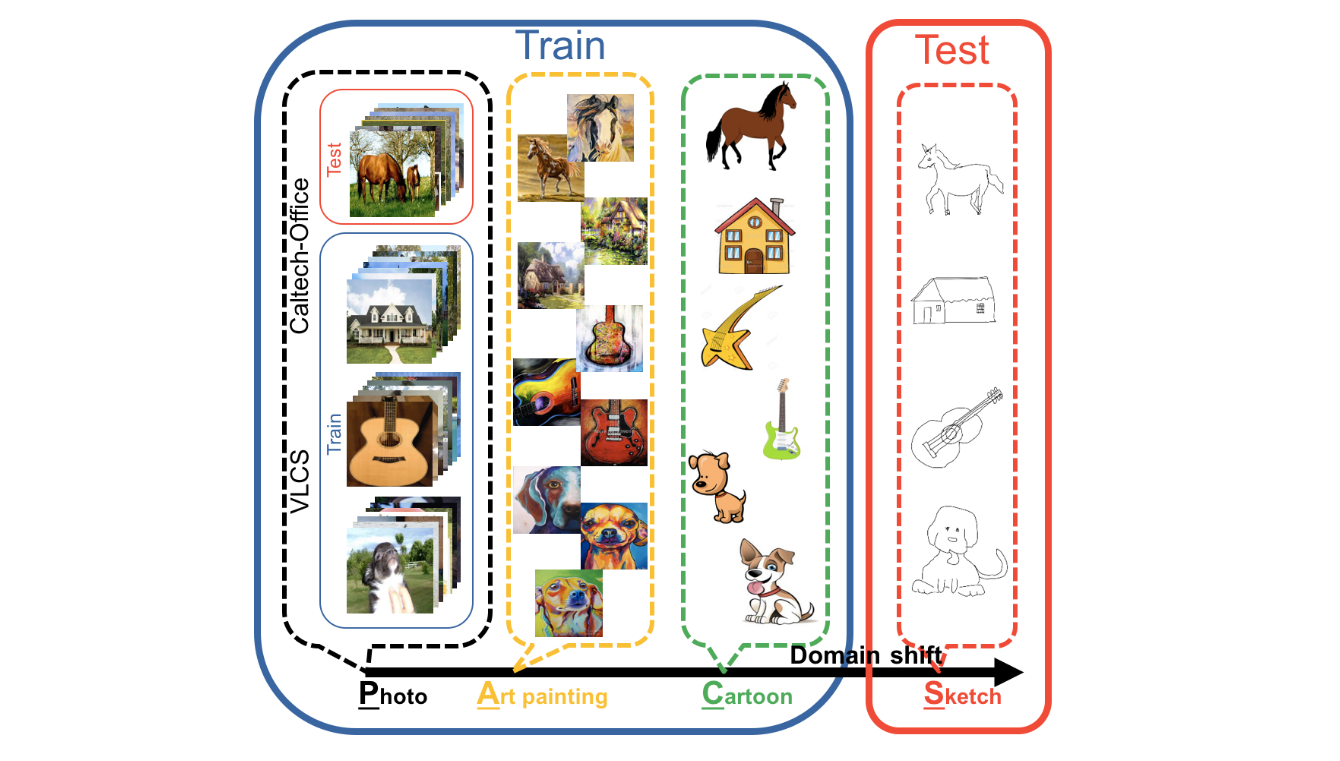
\includegraphics[width=\textwidth]{fig/PACS-dataset.png}
\end{frame}

\begin{frame}[t]{GBML vs Black-box adaptation}
  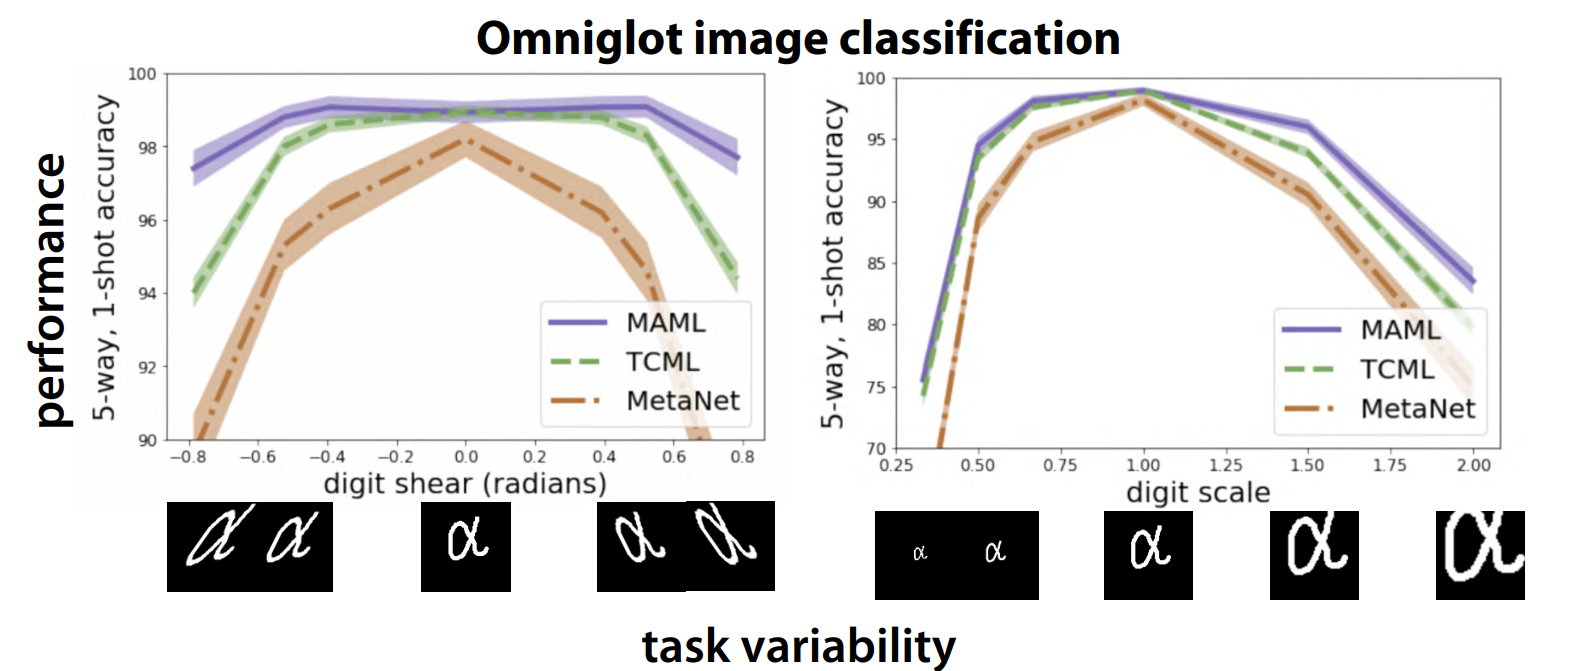
\includegraphics[width=\textwidth]{fig/gbml-ood.png}

  TCML: 就是 SNAIL
\end{frame}

\section{Domain Generalization in Meta Learning}

\begin{frame}{Formulation}
  \begin{itemize}
    \item $S$ source domains: $\mathcal{D}_1, \mathcal{D}_2, \cdots, \mathcal{D}_S$, $D_i \sim \mathcal{D}_i$
    \item target domain(s): $\mathcal{D}_T$
  \end{itemize}


  All of $D_i$ contains data pairs with same $\mathcal{X} \rightarrow \mathcal{Y}$ (same input and output dimension)

  \vspace{1em}

  Want: Train $\Theta$ on source domains, and such $\Theta$ can easily be fine-tuned on target domain\\
  (MAML's objective but consider \textbf{domain shift})
\end{frame}

\begin{frame}{Common task formulation strategies}
  在構造 meta-train tasks 時,train/test 刻意選來自不同 domain 的 batches or module
\end{frame}


\begin{frame}
  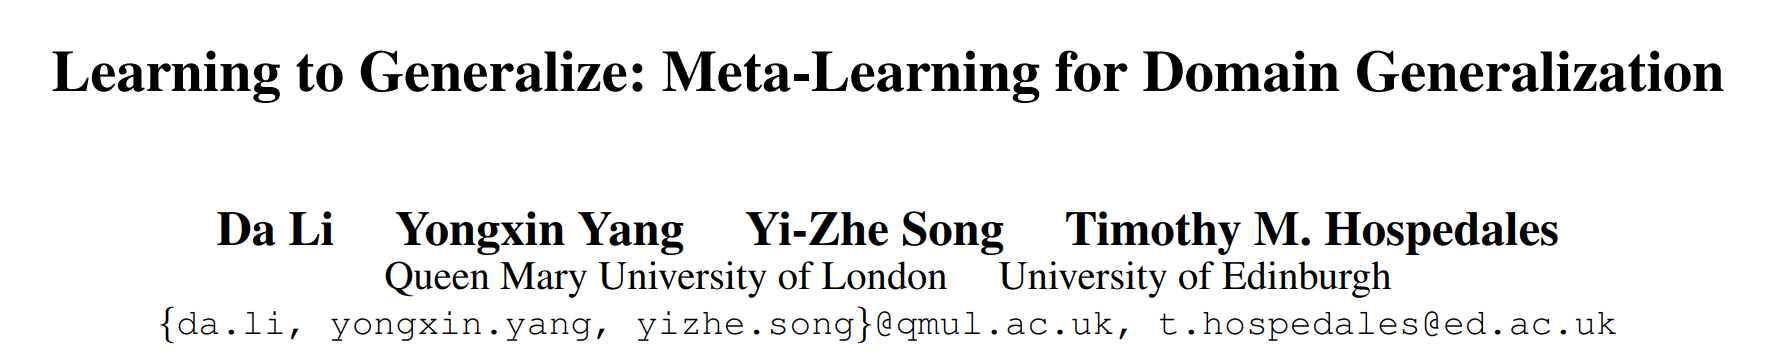
\includegraphics[width=\textwidth]{fig/MLDG-title.png}
  \center AAAI 2018
\end{frame}

\begin{frame}[t]{Idea}
  \begin{itemize}
    \item Meta-learn init parameters $\theta$
    \item Split $S$ into $\bar{S}$ (virtual meta-train), $\breve{S}$ (virtual meta-test)
  \end{itemize}

  \vspace{1em}
  \begin{block}{Meta Objective}
    
    \begin{itemize}
      \item $F(\theta) = \mathbb{E}_{D \sim \bar{S}} \frac{1}{N} \sum_{D} l_\theta(y, \hat{y})$
      \item $G({\color{red}{\theta^\prime}}) = \mathbb{E}_{D \sim \breve{S}} \frac{1}{N} \sum_{D} l_{\color{red}{\theta^\prime}} (y, \hat{y})$
      \item $\theta^\prime = \theta - \alpha \nabla_\theta F(\theta)$, one step here for example
      \item Final objective: $F(\theta) + \beta G(\theta - \alpha \nabla_\theta F(\theta))$
    \end{itemize}
  \end{block}
\end{frame}

\begin{frame}{Meta Objective}
  \begin{equation*}
      F(\theta) + \beta G(\theta - \alpha \nabla_\theta F(\theta))
  \end{equation*}

  To minimize the loss on training domains, also ensure the direction taken to achieve this also lead to improvment in virtual meta-test domain
\end{frame}

\begin{frame}{More detail about Meta Objective}
  \begin{equation*}
    \begin{aligned}
      & F(\theta) + \beta G(\theta - \alpha \nabla_\theta F(\theta))  \\
      &\approx F(\theta) + \beta[G(\theta) - \alpha \nabla_\theta G(\theta) \cdot \nabla_\theta F(\theta)] \\
      &= F(\theta) + \beta G(\theta) - \alpha \beta \underline{\nabla_\theta G(\theta) \cdot \nabla_\theta F(\theta)}
    \end{aligned}
  \end{equation*}
\end{frame}

\begin{frame}[t]{Other Regularizers}
  \begin{itemize}
    \item $F(\theta) + \beta G(\theta) - \alpha \beta \cos(\nabla_\theta F(\theta), \nabla_\theta G(\theta))$
    \item $F(\theta) + \beta ||\nabla_{\theta^\prime} (\theta - \alpha \nabla_\theta F(\theta))||_2$
  \end{itemize}

  \vspace{2em}
  Vanilla MLDG performs best in PACS dataset
\end{frame}

\begin{frame}
  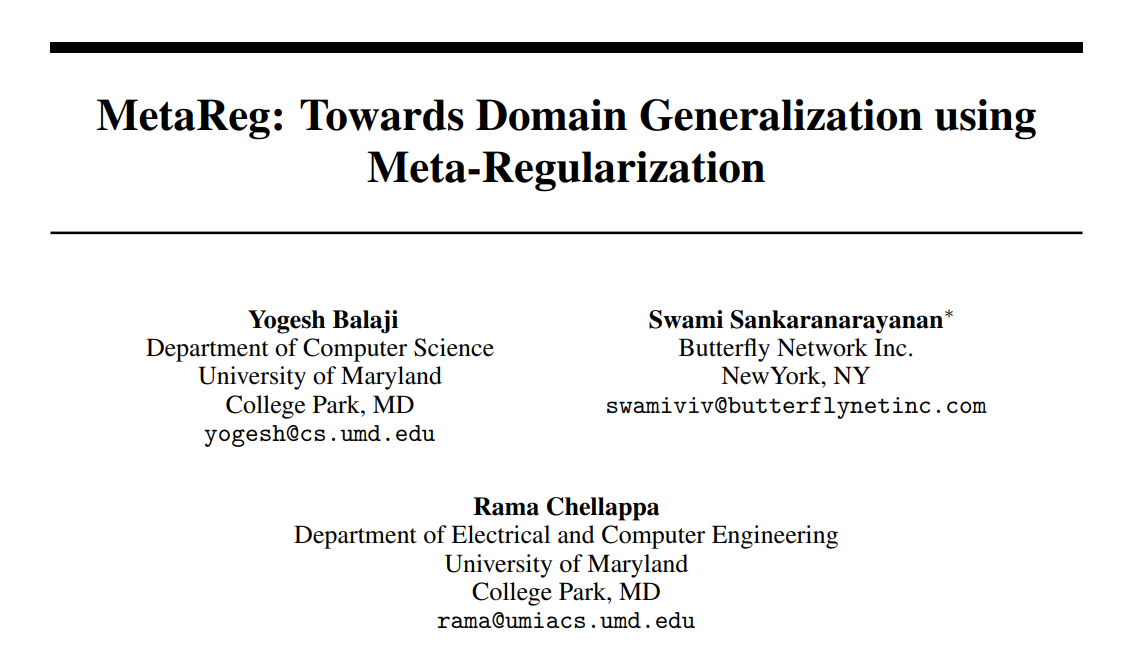
\includegraphics[width=\textwidth]{fig/MetaReg.png}
  \center NeurIPS 2018
\end{frame}

\begin{frame}{Idea}
  \begin{itemize}
    \item Meta-learn Domain Generalization (DG) regularizer $R_\phi$
    \item It's hard to hand-craft such regulaizer, so we learn it!
    \item Split model; param to $\psi, \theta$ (Note: no $\phi$ here)
      \begin{itemize}
        \item $\psi$: feature extractor
        \item $\theta$: task-specific network
      \end{itemize}
  \end{itemize}
\end{frame}

\begin{frame}{Network Arch.}
  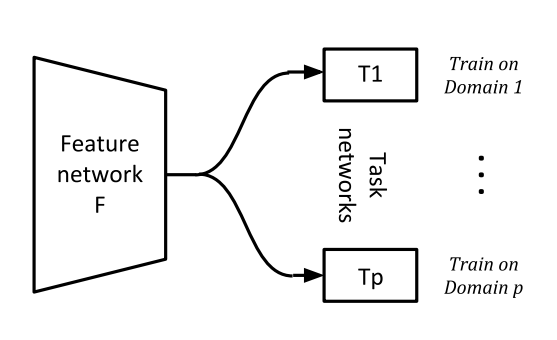
\includegraphics[width=\textwidth]{fig/meta-reg-arch.png}
\end{frame}

\begin{frame}{Algorithm Flow}
  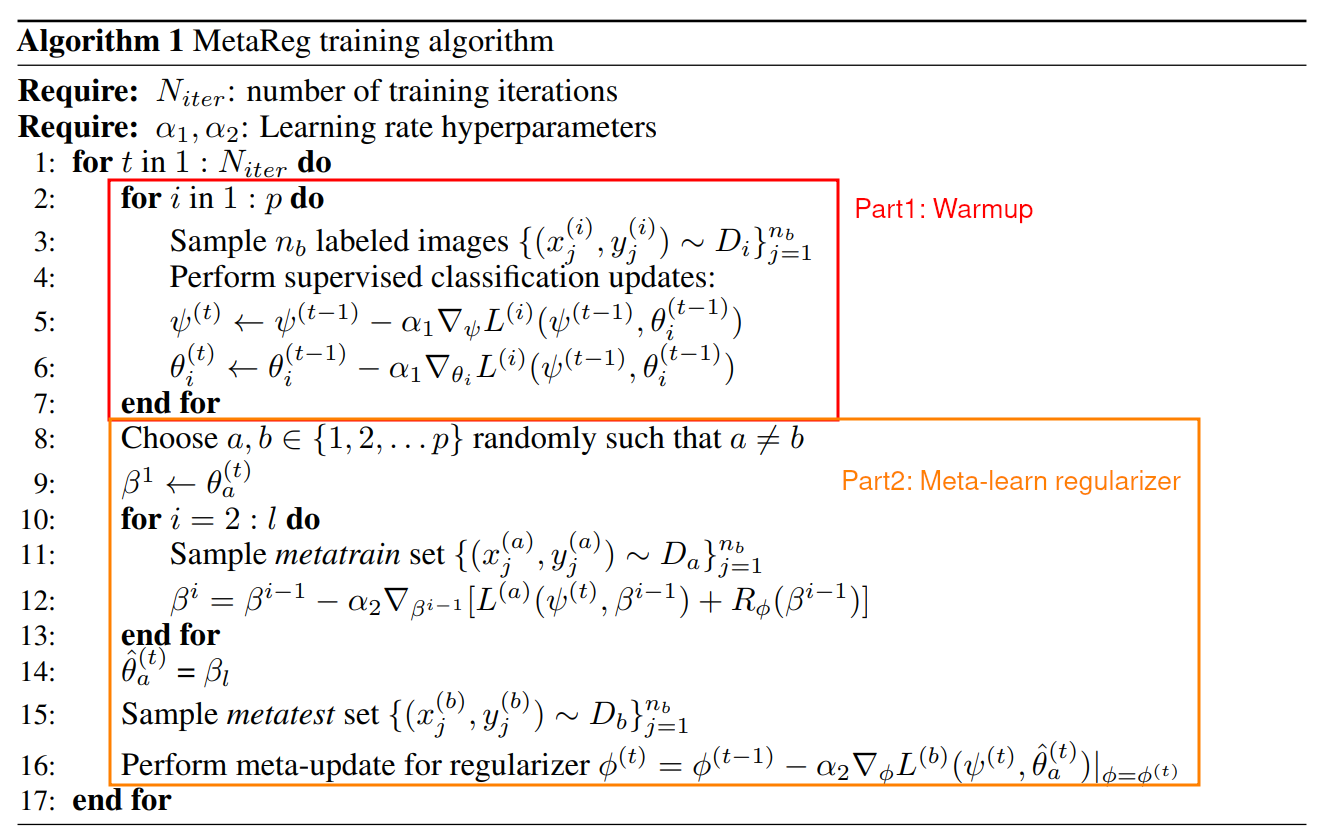
\includegraphics[width=\textwidth]{fig/meta-reg-alg.png}
\end{frame}

\begin{frame}{How to meta-learn regularizer}
  Note: In warmup stage, no regularization term when updating $\psi, \theta$

  \begin{block}{Part2: meta-learn $R_\phi$}
    \begin{enumerate}
      \item sample 2 domains $a,b$
      \item initialize $\theta_{\text{new}}^0 \leftarrow \theta_a$
      \item Update many steps using batches in $a$ with $R(\phi)$\\
        $\theta_{\text{new}}^t \leftarrow \theta_{\text{new}}^{t-1} - \alpha \nabla_{\theta_{\text{new}}^{t-1}}[L^{(a)}(\theta_{\text{new}}^{t-1}) + {\color{red}{R_\phi}(\theta_{\text{new}}^{t-1})}]$
      \item Update $\phi$ using batches in $b$\\
        $\phi \leftarrow \phi - \alpha \nabla_\phi L^{(b)}(\theta^T_{\text{new}})$
    \end{enumerate}
  \end{block}
\end{frame}

\begin{frame}{Part3: Fine-tune (Meta-test)}
  Retrain the model with one $F-D$ pair with $R_\phi$ as initial param
\end{frame}

\begin{frame}
  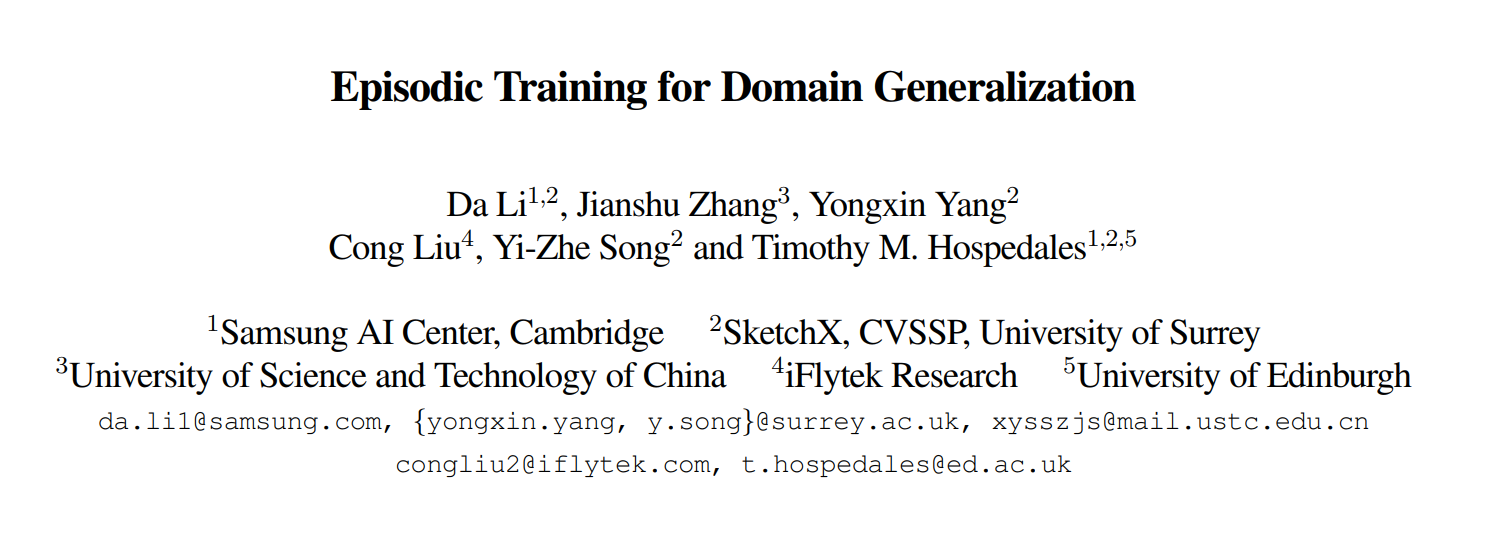
\includegraphics[width=\textwidth]{fig/EpiFCR-title.png}
  \center ICCV 2019
\end{frame}

\begin{frame}{Idea}
  \begin{itemize}
    \item Use mismatched feature encoder and task-specific network to enable DG
    \item 本文的 $\psi$ 和 $\theta$ 所代表的東西剛好反過來
      \begin{itemize}
        \item $\theta$: feature extractor
        \item $\psi$: task-specific network
      \end{itemize}
  \end{itemize}
\end{frame}

\begin{frame}{Network Arch.}
  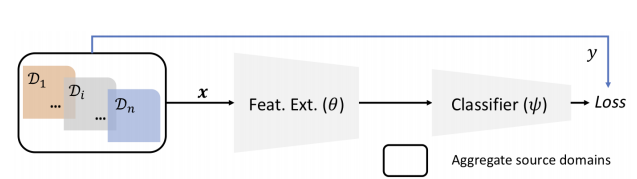
\includegraphics[width=.5\textwidth]{fig/epi-agg.png}
  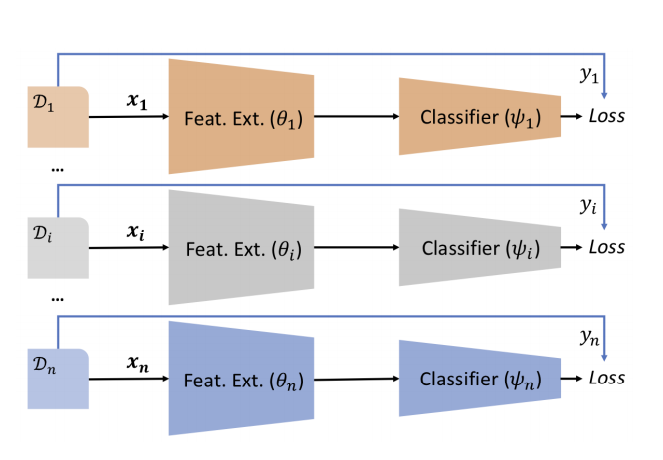
\includegraphics[width=.5\textwidth]{fig/epi-ind.png}
\end{frame}

\begin{frame}{Algorithm Flow}
  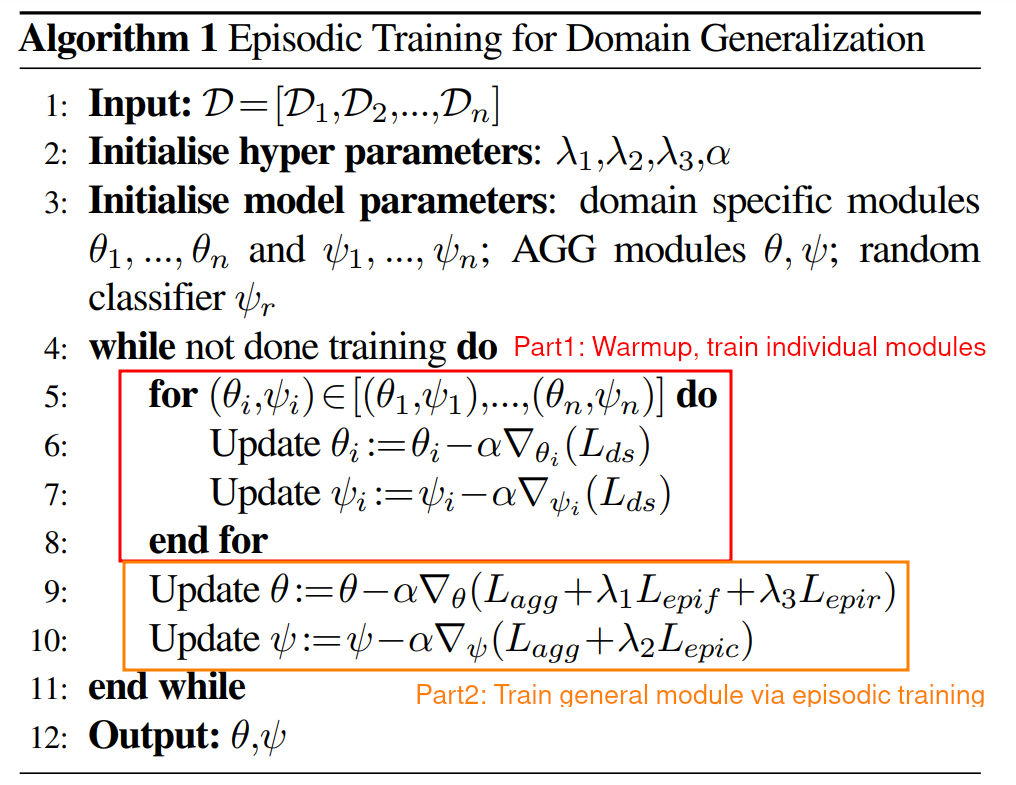
\includegraphics[width=.7\textwidth]{fig/epi-alg-flow.png}
\end{frame}

\begin{frame}{Part2: Episodic training for Feature Extractor $\theta$}
    Want to learn encoder that can encode $x$ from $a$ domain, can be classified well using $b$ domain's specific network
    \begin{equation*}
      \arg \min_\theta \mathbb{E}_{ a \neq b} [\mathbb{E}_{(x,y) \sim \mathcal{D}_a}(y, \psi_b({\color{red}{\theta(x)}}))] 
    \end{equation*}
    \vspace{1em}
    Can also be random specific network
    \begin{equation*}
      \arg \min_\theta \mathbb{E}_{a} [\mathbb{E}_{(x,y) \sim \mathcal{D}_a}(y, \psi_{\text{random}}({\color{red}{\theta(x)}}))] 
    \end{equation*}
    \vspace{1em}
    Note: $\psi_b$, $\psi_{\text{random}}$(?) is fixed when updating $\theta$
\end{frame}

\begin{frame}[t]{Part2: Episodic training for target network $\psi$}
  Want to learn target network that can process feature embedding for $x$ from $a$ domain using $b$ domain's feature extractor

  \begin{equation*}
    \arg \min_\theta \mathbb{E}_{ a \neq b} [\mathbb{E}_{(x,y) \sim \mathcal{D}_a}(y, {\color{red}{\psi}}(\theta_b(x)))] 
  \end{equation*}
    Note: $\theta_b$ is fixed when updating $\psi$
\end{frame}

\begin{frame}{Part3: Fine-tune (Meta-test)}
  Use $\theta, \psi$ as init param for target domain
\end{frame}

\begin{frame}[t]{Experiments on PACS dataset}
  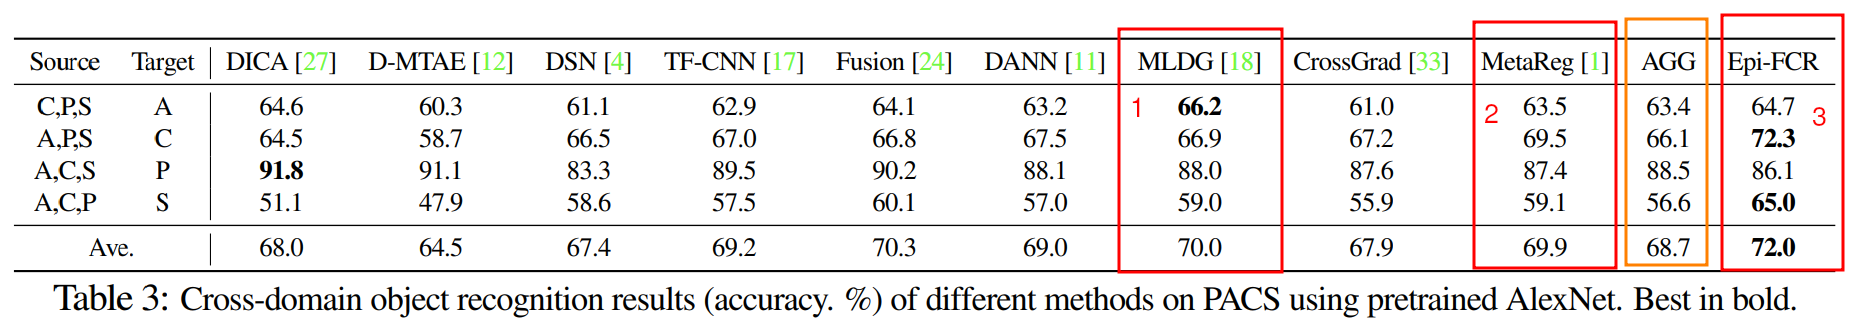
\includegraphics[width=\textwidth]{fig/pacs-exp.png}
\end{frame}

\begin{frame}{Conclusion \& Future work}
  \begin{itemize}
    \item Use batches from different domains during episodic training
    \item Still depend on the diversity of source domains (好像是廢話 :p)
    \item Will apply those techniques in MetaASR (ICASSP 2020)
        \begin{itemize}
          \item MLDG (第一篇) doesn't improve 
          \item Switch the setting from cross-language to cross-accent (HKUST in early March)
        \end{itemize}
  \end{itemize}
\end{frame}

\begin{frame}
	\begin{center}
    %\weib{\LARGE{謝謝聆聽!}}
    \LARGE{Questions?}
	\end{center}
\end{frame}

\end{document} 
